\section{Template-based Programming model}
\label{sec:model}

\begin{figure}[htb]
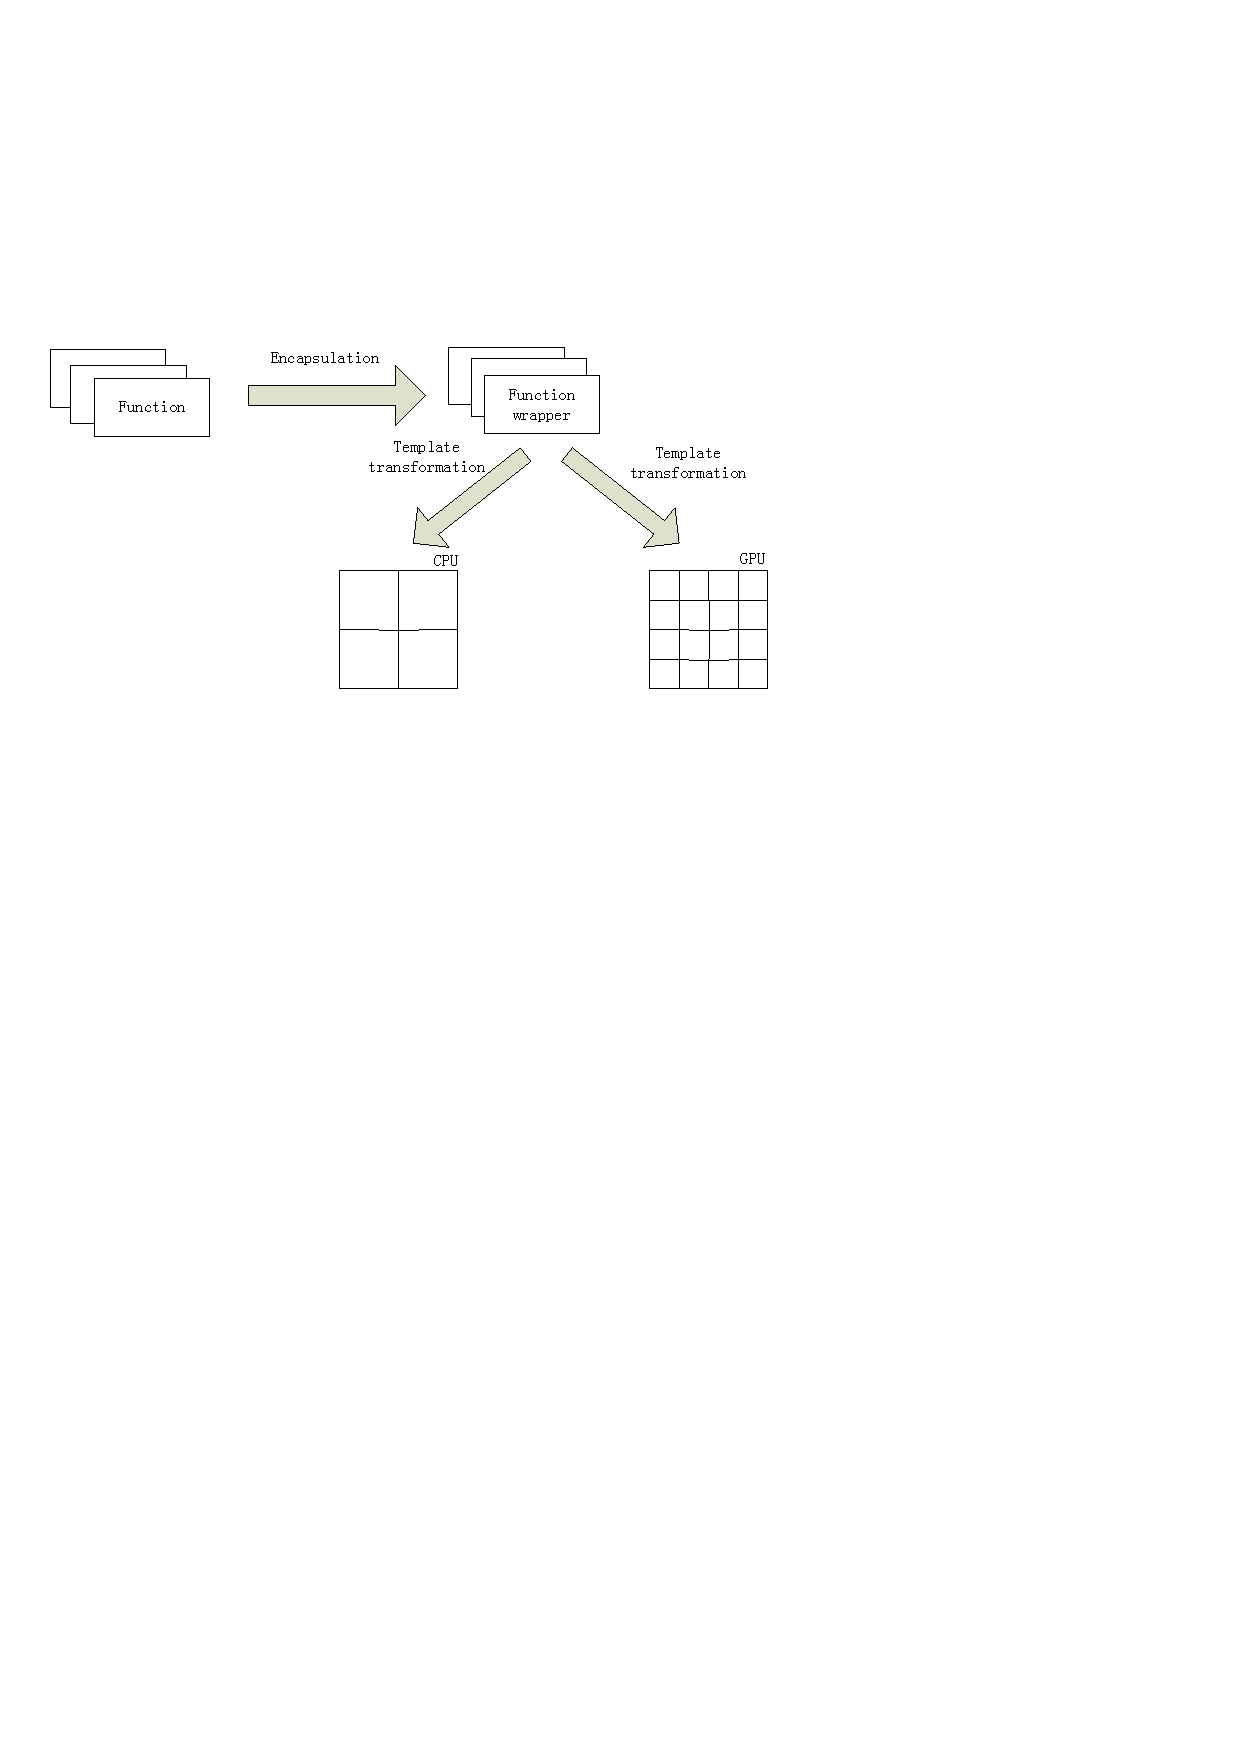
\includegraphics[width=3.3in]{../overview}
\caption{Overview of template-based programming model: Programmers
write side-effect free functions in C/C++, then encapsulate them in
function wrappers. Template library regards a function wrapper as
a task, which is automatically transformed into a
group of subtasks based on appropriate parallel patterns. Finally,
subtasks directly run on physical multicores.}
\label{fig:overview}
\end{figure}

We propose a template metaprogramming approach to support parallel programms
running on different multi-core systems. \reffig{overview} gives an overview
of our approach: a side-effect free function is abstracted as a \emph{task}
and is wrapped in a \emph{function wrapper}. We provide wrappers
to support different parallel patterns:

\begin{itemize}
\item \textbf{Hierarchy pattern.} A task is recursively divided into subtasks
and subtasks can execute on multiple cores in parallel.

\item \textbf{Pipeline pattern.} A task is divided into a series of processing
subtasks, where the output of a previous subtask is directly used as the input
of the next subtask and each subtask execute on a core.

\item \textbf{Map-Reduce pattern.} A task is divided into a map phase and a
reduce phase, where subtasks in each phase can execute in parallel on multiple
cores. The input of reduce phase is the output of the map phase.

\end{itemize}

The transformation from a function wrapper to parallel patterns is a
source-to-source conversion with C++ templates, which are called \emph{TF
class} in this paper (Section~\ref{sect:tf}).  The converted code calls
architecture-specific building block classes (Section~\ref{sect:bb}) so that
when compiled, a task can execute on
different multi-core systems in parallel at run time. 

The rest of this section first describes three class types of our approach, i.e.,
TF, view, and building block classes. 
%(1) View class, a representation of underlying containers such as vector or matrix.
%(2) Building block class,
%provide basic executions of tasks on multicores (3) TF class, each one
%represents a parallel pattern. 
To illustrate the usage of our template library, we then describe two examples
using these three types of classes.

\subsection{TF Class}
\label{sect:tf}

A \textit{TF class} (short name for \textit{TransFormation class}) is a template
class representing a parallel pattern which transforms a task to a group of
subtasks in isomorphism. In other words, the transformed task has the same interface
while owns a call graph inside to complete the original computation by a
group of subtasks. Specifically, the following two classes are used in this paper: 

\begin{itemize} 
\item \textbf{TF\_hierarchy}. This template class recursively divides a task into subtasks
until certain predicate is evaluated as true. %As Fig.~\ref{fig:mmexample} depicted,  we use
In fact, TF\_hierarchy can implement a programming model similar to Sequoia and
we use TF\_hierarchy to implement both hierarchy and Map-Reduce pattern.

\item \textbf{TF\_pipeline}. This template class synthesizes a call chain of an
arbirary number of functions into a pipeline. This is a common pattern for
stream kernel programming model.
\end{itemize} 


%A side-effect free function is referred to as \emph{task} in libvina. As a rule of thumb,
In this paper, we consider a class of computation-intensive functions (or tasks) that are 
self-contained, i.e., external data references are limited and
calling graphs of them are simple. For these functions, it's possible to
decouple a task into a cluster of subtasks. These subtasks are identical
except for arguments and we can distribute subtasks on multi-core to execute simultaneously. 

%We implement two TF classes in libvina though  it is not
%necessary to use TF classes to perform source transformations. We
%encourage to do so because it has engineering advantages, which reduces
%effects of system programmers.



\subsection{View class}

A \emph{View} is a class representing a subset of container's data. For example,
a matrix type could have views that contains a subset of elements of a matrix.
There are two kinds of views, \emph{ReadView} and \emph{WriteView}.
A ReadView is read-only, while a WriteView allows write operations on its data
(by providing interfaces to write). 

To ensure multi-thread safety, \emph{ReadViewMT} and \emph{WriteViewMT} are
defined. For these two types, each object contains a signal that is copied across multiple
threads. All operations of ReadViewMT or WriteViewMT are blocked until the
current thread is signaled by other threads.

\reffig{view} depicts the relationship of views. Concrete lines means that
a type cast from a source node to a destination node is legal, i.e., an implicit
conversion in C++.  Dashed lines means a source node can generate objects of
the type of the destination node. Labels on the dashed line signifies how
signals are created or copied.
Shadow region is another thread space.

%The only approach to communicate with other
%threads is through a special kind of view called \emph{ViewMT}.  

The design of view class has two purposes. 1) The classes are type-safed.
Because template instantiation is not visible for programmers, our
source transformations by templates could introduce subtle errors. We
expect compilers complain explicitly when unintentional
transformations happen. 2) View classes hide communication details. 
Implementations have choice to optimize data movement according to
architectures. Shared memory systems~\cite{larrabee} and communication-exposed multicores~\cite{cellbe, imagine} usually have different strategies to perform
the operations.

\begin{figure}
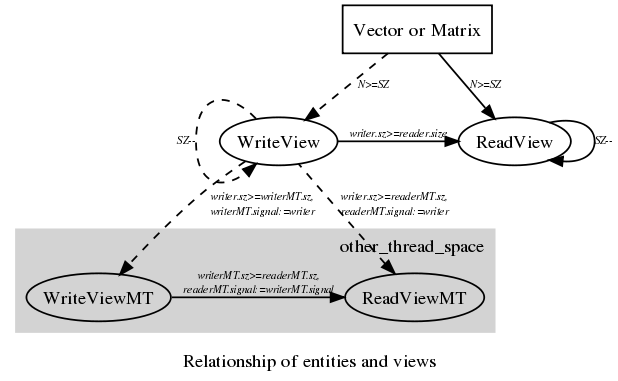
\includegraphics[width=3.6in]{../relationship_views}
\caption{The relationship of view classes. A concrete line represents a valid
   type cast, while a dashed line represents a source node can generate objects
of the type pointed to. Labels specify how signals are created or copied
across views.}
\label{fig:view}
\end{figure}


\subsection{Buiding block class}
\label{sect:bb}

\begin{table}[hbt]
\caption{Build block classes in libvina}
\begin{tabular}{|c|l|l|}
\hline
Name& Semantics& Usage Example\\
\hline
\textbf{par$<$T, K, F$>$}& Iterate function \textit{F} \textit{K} times &par$<$\_tail, 4, F$>$\\ 
                         &in parallel, implicit barrier                 &::apply();\\                
\hline
\textbf{seq$<$T, K, F$>$}& Iterate function \textit{F} \textit{K} times&seq$<$\_tail, 5, F$>$\\
                         &                                             &::apply();\\
\hline
\textbf{reduce$<$K, F$>$}&Reduce \textit{K} values using &reduce$<$8, F$>$\\
&function
\textit{F}&::apply(values)\\
\hline
\textbf{mt::thread$<$F$>$}&Spawn a thread to execute  & mt::thread$<$F$>$\\
                          &function \textit{F}        & ::apply();\\
%\textbf{do\_}&loop until predicate is evaluated true.& 
\hline
\end{tabular}\label{tbl:bb}
\end{table}

A building block class is a high-level abstraction of execution patterns that
hide architecture-specific details. Programmers can use building blocks to
execute tasks on different multi-core platforms.
\reftable{bb} lists building blocks in libvina. For tasks that can
executed in SPMD (Single-Program-Multiple-Data) fasion, \code{par} class spawns
multiple threads to execute subtasks in parallel. \code{seq} class supports
pipeline patterns. Parameter $T$ in \code{par} or \code{seq} could be nested
\code{par}, nested \code{seq}, or \code{\_tail} (meaning no further nestings).
For instance, we can write the following statement 

%However, if it is
%not the case, we have to deal with dependences carefully using \code{seq} and \code{reduce}. 
%Like traditional programming languages, our
%building blocks of iterations support nesting definition. In addition, both \textit{seq} and
%\textit{par} are interoperable. 

\begin{lstlisting}
seq<par<_tail, 4>, 3, F>::apply();
\end{lstlisting}
to build to a two-level loop, and the nested loop are executed in
parallel. The equivalent OpenMP code is:
\begin{lstlisting}
F f;
int i, j;
for (i=0; i<3; ++i)
{
  #pragma omp parallel private(j)
  for (j=0; j<4; ++j) 
    f(i, j);
}//implicit barrier
\end{lstlisting}

%The first template parameter $T$ of iterations is used to support nest. It could be
%either a par or a seq. Special classes \code{par\_tail} and \code{seq\_tail} are
%symbols to indicate the end of nest.

The \code{reduce} class supports the ``reduce" pattern in MapReduce style tasks.
Specifically, a given function $F$ is used to reduce $K$ input values and the
final result is stored in the first value. Note that many of the $K-1$ times
reduce operations are executed in parallel using multiple threads.

Finally, \code{mt::thread} class provides a thread interface for programmers to
dynamically spawn a new thread to execute a function.

%can exploit it to bind thread directly (\textit{e.g.} line 19 of List 2)
%or develop other customized building blocks.



%programming model
\comment{
We use template metaprogramming to implement a parallel programming model.
Essentially, our approach utilizes C++ template mechanism to
perform source-to-source transformations for multicores. Side-effect
free functions are abstracted as \emph{tasks}. A task is
wrapped in the form of template class, named \emph{function
  wrapper}.  A \emph{TF class} is a template class, which
is capable of transforming a task into a group of subtasks based on
a parallel pattern. Tasks
apply TF classes according to their appropriate
parallel patterns. This process is called ast \emph{adaption}. 
Finally, we use \emph{building block classes} to define executions of tasks
on specific architectures. Both TF classes and building
blocks are organized as a library --
\textbf{libvina}. Fig.~\ref{fig:overview} depicts the diagram of template
library-based programming model. Conventional functions are
encapsuated into function wrappers. After transformation at compile time, they are
executed on different multicore architectures at run time.
}

\subsection{Example I: Hierarchy Pattern}

\renewcommand\linenumberfont{\normalfont\small}
\setlength\linenumbersep{-0.06in}

\begin{figure}[hbt]
  \inputsrc{sgemm.cc}
  \caption{Source code of matrix multiplication (class SGEMM) using hierarchy pattern.}
  \label{fig:sgemm}
\end{figure}

\reffig{sgemm} is the source code for matrix multiplication by adapting \code{TF\_hierarchy}
to implement a \emph{Divide-and-Conquer} algorithm. 
Function \code{innner} at line 20 divides task into subtasks, while function \code{leaf} at
line 45 performs
computation. Call operator function at line 14 is the user interface for the task.
Line 24$\sim$37 is lambda expression to perform map/reduce.
%, corresponding to SGEMM(512, 512, 512) node in \reffig{mmexample}.

To leverage static information, libvina need to
associate template parameters with ADTs' parameters. For example, 
Matrix class cantains 3 template paramters: type, the number of
row, the number of column. A definition of Matrix is at line 26 of
\reffig{sgemm}. 

Line 30$\sim$32 of \reffig{sgemm} generate subviews by calling functions.

\reffig{mmexample} illustrates ...

%Programmers using our template-based programming model are free to
%choose ways to parallelize tasks. An example of applying 
%Sequoia's programming model is shown in Fig.~\ref{fig:mmexample}. 
%\textit{sgemm} is a task to perform matrix-mulitplication. 
%We can apply a TF class dedicated to hierarchical division.  \reffig{sgemm}
%illustrates the adaption. As a reuslt, we
%implement the straightforward \emph{Divide-and-Conquer} algorithm for
%sgemm, which divides a matrix into K*K
%submatrices, computes them recursively, and reduces the results for
%each division.
%The control flow of source transformation is programmed
%using template metaprogramming inside of the TF class. 

\begin{figure}[htb]
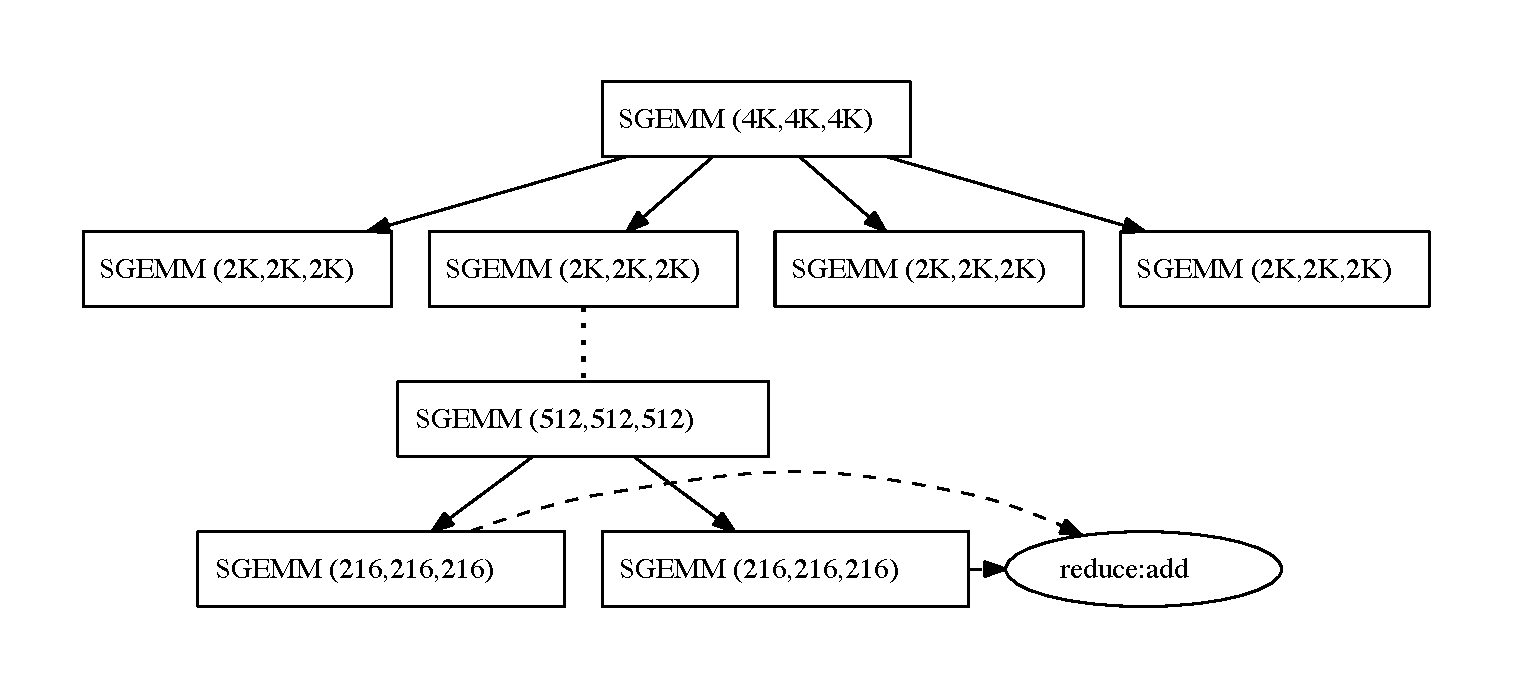
\includegraphics[width=3.5in]{../mmexample}
\caption{An illustration of recursively dividing the task of matrix multiplication
into subtasks. The original task
is automatically divided into a number of subtasks at compile time.
The division is implemented in \reffig{sgemm}. Here the parameter $K$ is set to 2.
As a result, each task is divided into 4 subtasks.
%Triple in figure represents
%task parameters (M, P, N), which means A[M][P] * B[P][N]. The figure
%is the result of parameterizing K = 2.
}
\label{fig:mmexample}
\end{figure}


\subsection{Example II: Pipeline Pattern}

\begin{figure}[hbt]
  \inputsrc{langpipe.cc}
  \caption{Source code of a pipeline pattern (langpipe).}
  \label{fig:pipe}
\end{figure}
%code of langpipe: A translation is a standalone function wrapper. TF class synthesizes a pipeline. 

%Building blocks \textit{par} and \textit{reduce} to express execution.
\reffig{pipe} gives pipeline processing example, which is similar to Streamit.
It implements language translation pipeline by
synthesizing a pipeline of four standalone functions. \code{TF\_pipeline} is a TF class
representing time-multiplex parallelism. As shown in examples,
the parallel patterns and execution models are dramatically
different, however, our approach can describing them well in uniform
language constructs.

%meaning
Our programming model facilitates the separation of roles in software
development. Algorithm-centric programmers are only concerned of algorithm
in conventional C/C++ form, as at line 45 of List 1 and line 8 of
List 2. On the other side,  system programmers knowing underlying
architectures are in charge of developing and
applying template classes to specialize tasks for the specific
targets. This separation not only simplifies the difficulties of writing and
tuning parallel programs, but also facilitates to develop effecient and
portable programs for various multicores.

